% drafts/appendix-c-counterexample.tex — Monotonicity Counterexample

We present the full computation showing that Construction~A fails on
the balanced ternary tree with $n = 8$.

%%====================================================================
\subsection*{Tree structure}

The balanced ternary tree on 8 nodes has root label~4 and the
following adjacency:
\begin{center}
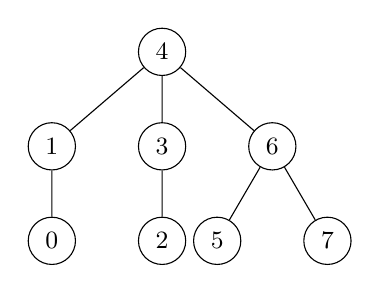
\begin{tikzpicture}[
  level distance=12mm, sibling distance=14mm,
  every node/.style={circle,draw,minimum size=6mm,inner sep=0pt,
    font=\small}
]
\node {4}
  child { node {1}
    child { node {0} }
  }
  child { node {3}
    child { node {2} }
  }
  child { node {6}
    child { node {5} }
    child { node {7} }
  };
\end{tikzpicture}
\end{center}

This tree is \emph{not} index-monotonic: node~7 has parent~6,
violating the condition $\text{label}(\text{parent}) >
\text{label}(\text{child})$ since $6 < 7$.

%%====================================================================
\subsection*{Index sets from Construction~A}

Applying the generic index-set computation:
\begin{center}
\begin{tabular}{@{}clll@{}}
\toprule
$j$ & $\Uset{j}$ & $\Rset{j}$ & $\Occ{j}$ \\
\midrule
0 & $\{1, 4\}$       & $\emptyset$     & $\{0\}$ \\
1 & $\{4\}$           & $\{0\}$         & $\{0, 1\}$ \\
2 & $\{3, 4\}$       & $\{1\}$         & $\{2\}$ \\
3 & $\{4\}$           & $\{1, 2\}$     & $\{2, 3\}$ \\
4 & $\emptyset$       & $\{1, 3\}$     & $\{0,1,2,3,4,5,6,7\}$ \\
5 & $\{6, 4\}$       & $\{1, 3\}$     & $\{5\}$ \\
6 & $\{4\}$           & $\{1, 3, 5\}$ & $\{5, 6, 7\}$ \\
7 & $\{6, 4\}$       & $\{1, 3, 5\}$ & $\{7\}$ \\
\bottomrule
\end{tabular}
\end{center}

%%====================================================================
\subsection*{Majorana operators (partial)}

From these index sets, the Majorana operators for modes 4 and~7 are:
\begin{align*}
  c_4 &= -Y_1 Y_3 X_4 Z_5 Z_6 Z_7, \\
  d_4 &= Y_1 Y_3 Y_4 Z_5 Z_6 Z_7, \\
  c_7 &= -Y_1 Y_3 Y_5 X_6 X_7, \\
  d_7 &= Y_1 Y_3 Y_5 X_6 Y_7.
\end{align*}
(Operators on unlisted qubits are identity.)

%%====================================================================
\subsection*{Failed anticommutator}

Computing $\acomm{\an{4}}{\ad{7}}$, where
$\an{4} = \frac{1}{2}(c_4 + i\,d_4)$ and
$\ad{7} = \frac{1}{2}(c_7 - i\,d_7)$:

\begin{align*}
  \acomm{\an{4}}{\ad{7}}
    &= \tfrac{1}{4}\bigl[
      \acomm{c_4}{c_7} + i\,\acomm{d_4}{c_7} \\
    &\quad\quad\;  - i\,\acomm{c_4}{d_7} + \acomm{d_4}{d_7}
    \bigr].
\end{align*}

For a valid encoding, this should vanish ($4 \neq 7$).  Instead:
\begin{align*}
  \acomm{c_4}{c_7} &= -2\,ZZZZZIZZ, \\
  \acomm{d_4}{d_7} &= +2\,ZZZZZIZZ, \\
  \acomm{c_4}{d_7} &= -2i\,ZZZZZIZZ, \\
  \acomm{d_4}{c_7} &= -2i\,ZZZZZIZZ.
\end{align*}

These do \emph{not} cancel in the linear combination:
\begin{equation*}
  \acomm{\an{4}}{\ad{7}} = (0.5i)\; ZZZZZIXY + (-0.5)\; ZZZZZIXX
    \neq 0.
\end{equation*}

%%====================================================================
\subsection*{Diagnosis}

The failure arises because nodes~6 and~7 share the parent--child
edge with $\text{label}(6) < \text{label}(7)$.  In the remainder-set
computation for $j = 7$:
\[
  \Rset{7} = \{v : v \text{ is a child of an ancestor of } 7,\;
    v < 7,\; v \notin \text{path}(7)\} = \{1, 3, 5\}.
\]
The $Z$-operators placed on qubits $\{1, 3, 5\}$ via the remainder
set of mode~7 overlap with $\Uset{4} = \emptyset$ and $\Rset{4} =
\{1, 3\}$, creating cross-mode interference in the anticommutator.
For a star tree, all remainder sets consist only of siblings, which
never overlap with update or occupation sets of other modes.

%%====================================================================
\subsection*{Verification by Construction~B}

Applying Construction~B (path-based encoding,
\cref{sec:tree-encoding}, \cref{sec:constructions}) to the \emph{same} balanced ternary tree
produces Majorana operators that satisfy \emph{all} $\binom{16}{2} =
120$ anticommutation relations exactly.  The tree topology is not the
problem; the index-set derivation method is.
